\documentclass[a4paper,11pt]{article}

\usepackage[utf8]{inputenc}
\usepackage[T1]{fontenc}
\usepackage{geometry}
\geometry{margin=2.2cm}
\usepackage{xcolor}
\usepackage{graphicx}
\graphicspath{{figures/}}
\usepackage{tikz}
\usetikzlibrary{calc}
\usepackage{everypage}
\usepackage{background}
\usepackage{amsmath}
\usepackage{amssymb}
\usepackage{booktabs}
\usepackage{caption}
\usepackage{float}
\usepackage[colorlinks=true,linkcolor=blue,urlcolor=blue]{hyperref}

\setlength{\parskip}{0.6em}
\setlength{\parindent}{0pt}

\definecolor{bordercolor}{RGB}{68,94,114}

\backgroundsetup{
  scale=1, color=bordercolor, opacity=1, angle=0,
  position=current page.center,
  contents={
\begin{tikzpicture}[remember picture, overlay]
    \draw[line width=4pt, color=bordercolor]
      ($(current page.south west) + (1cm,1cm)$) rectangle
      ($(current page.north east) - (1cm,1cm)$);
  \end{tikzpicture}}
}

\begin{document}

\begin{titlepage}
\thispagestyle{empty}
\centering
\vspace*{3cm}
{\Huge\bfseries IFRS 9 Expected Credit Loss Pipeline\\\bigskip
\LARGE PD $\times$ LGD $\times$ EAD across Macro Scenarios
\par}
\vspace{1.5cm}
{\Large Magnus Foldeström\par}
\vfill
\end{titlepage}

\section{What this project does}

Expected Credit Loss (ECL) under IFRS 9 is the accounting provision
for future credit losses on a lending portfolio. It combines the
three components estimated in the sibling projects into a single
provision number:
$$\mathrm{ECL} = \sum_{s \in \mathrm{scenarios}} w_s \cdot \mathrm{PD}_s \cdot \mathrm{LGD}_s \cdot \mathrm{EAD} \cdot \mathrm{DiscountFactor}.$$

This project runs the full IFRS 9 pipeline on a synthetic retail
portfolio of 50\,000 performing loans with total exposure of 3.78
billion EUR across five products (mortgage, auto, personal loan,
credit card, overdraft). It applies stage classification, applies
three probability-weighted macro scenarios, and produces the
provision number that would post to the balance sheet.

\section{Data}

\subsection{Portfolio}

\begin{table}[H]
\centering
\begin{tabular}{l r r r r}
\toprule
\textbf{Product} & \textbf{Loans} & \textbf{Mean PD 12m} & \textbf{Mean LGD} & \textbf{Total EAD (m EUR)} \\
\midrule
Mortgage       & 17\,411 & 2.6\%  & 22\% & 3\,399.5 \\
Auto           & 7\,581  & 4.9\%  & 43\% & 167.7 \\
Personal loan  & 10\,062 & 8.2\%  & 71\% & 112.1 \\
Credit card    & 9\,865  & 9.6\%  & 71\% & 71.6 \\
Overdraft      & 5\,081  & 12.3\% & 71\% & 29.7 \\
\bottomrule
\end{tabular}
\caption{Portfolio characteristics by product. Mortgages dominate EAD
by an order of magnitude despite lower default rates; unsecured
revolving products carry high PD and LGD but small balances.}
\end{table}

\subsection{Macro scenarios}

\begin{table}[H]
\centering
\begin{tabular}{l r r r r r}
\toprule
\textbf{Scenario} & \textbf{Weight} & \textbf{PD mult.} & \textbf{LGD mult.} & \textbf{Unemp \%} & \textbf{HPI YoY \%} \\
\midrule
Baseline        & 60\% & 1.00 & 1.00 & 7.5  & +2.5 \\
Adverse         & 30\% & 1.60 & 1.20 & 9.0  & -2.0 \\
Severe adverse  & 10\% & 2.40 & 1.50 & 11.5 & -6.0 \\
\bottomrule
\end{tabular}
\caption{Three probability-weighted macro paths. Multipliers are
applied to per-loan PD and LGD before ECL calculation, then
scenario-level ECLs are combined by weight to produce the final
IFRS 9 provision.}
\end{table}

\section{Methodology}

\subsection{IFRS 9 staging}

\begin{itemize}
  \item \textbf{Stage 1:} performing loans with no significant
        deterioration since origination. ECL is 12-month PD $\times$
        LGD $\times$ EAD, discounted one year.
  \item \textbf{Stage 2:} significant deterioration
        (credit-score drop $\geq$ 60 points OR watchlist flag) OR
        DPD between 30 and 89 days. ECL is lifetime.
  \item \textbf{Stage 3:} DPD $\geq$ 90 days (credit-impaired). PD
        set to 1; ECL is lifetime LGD $\times$ EAD.
\end{itemize}

The performing portfolio in this project shows 76.3\% in stage 1,
23.0\% in stage 2, and 0.8\% in stage 3.

\subsection{Lifetime PD}

Lifetime PD across remaining maturity $T$ (5 years for term loans,
3 years for revolving) is computed under a constant-hazard
assumption:
$$\mathrm{PD}_\mathrm{lifetime} = 1 - (1 - \mathrm{PD}_{12m})^T.$$

\subsection{Discounting}

Cash flows are discounted at an effective annual rate of 3\%. For
lifetime ECL the discount factor is the average of annual factors
across the remaining maturity.

\section{Results}

\subsection{Portfolio ECL under three scenarios}

\begin{table}[H]
\centering
\begin{tabular}{l r r}
\toprule
\textbf{Scenario} & \textbf{ECL (m EUR)} & \textbf{Coverage vs EAD} \\
\midrule
Baseline        & 77.5  & 2.05\% \\
Adverse         & 132.5 & 3.51\% \\
Severe adverse  & 217.9 & 5.77\% \\
\midrule
\textbf{Weighted (final IFRS 9 provision)} & \textbf{108.0} & \textbf{2.86\%} \\
\bottomrule
\end{tabular}
\caption{Portfolio ECL across the three macro scenarios and the
probability-weighted final provision. The adverse scenario adds
+71\% over baseline; severe adverse adds +181\%. Weighting brings
the final provision to 108m EUR, dominated by the 60\% baseline
contribution but lifted by the tail scenarios.}
\end{table}

\begin{figure}[H]
\centering
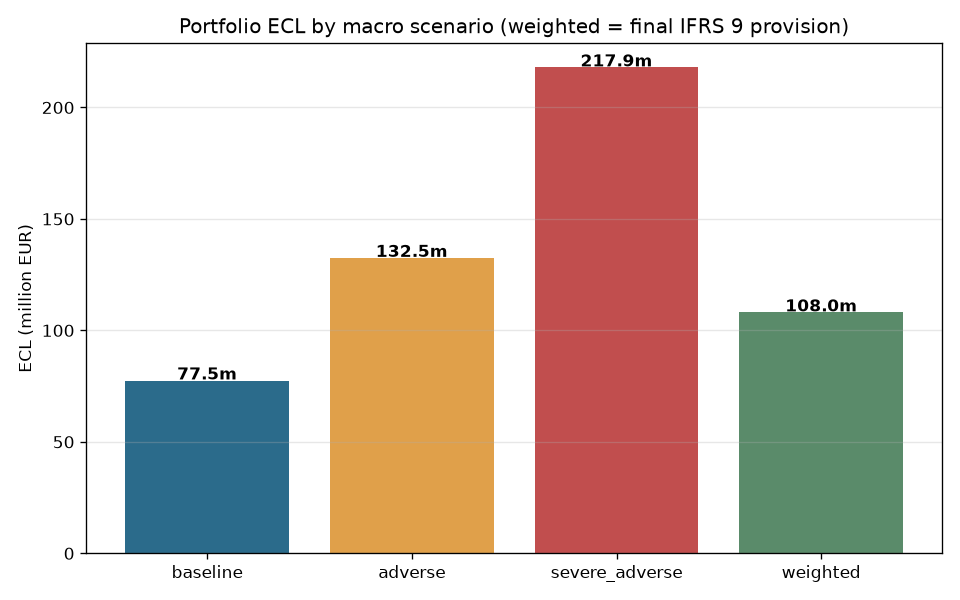
\includegraphics[width=0.9\textwidth]{01_ecl_by_scenario.png}
\caption{Portfolio ECL under each scenario and the weighted final
provision. The weighted number is what gets posted to the balance
sheet as impairment allowance.}
\end{figure}

\subsection{ECL by IFRS 9 stage}

\begin{table}[H]
\centering
\begin{tabular}{r r r r r}
\toprule
\textbf{Stage} & \textbf{Loans} & \textbf{Total EAD (m)} & \textbf{Weighted ECL (m)} & \textbf{Coverage} \\
\midrule
1 & 38\,140 & 2\,881.7 & 31.7  & 1.10\% \\
2 & 11\,483 & 868.2   & 67.8  & 7.81\% \\
3 & 377     & 30.7    & 8.6   & 28.05\% \\
\bottomrule
\end{tabular}
\caption{ECL split by IFRS 9 stage. Stage 2 alone carries 63\% of the
total weighted provision despite representing only 23\% of loan
count and 23\% of EAD, reflecting the lifetime-versus-12-month
difference. Stage 3 has the highest coverage ratio because
$\mathrm{PD} = 1$ by construction.}
\end{table}

\begin{figure}[H]
\centering
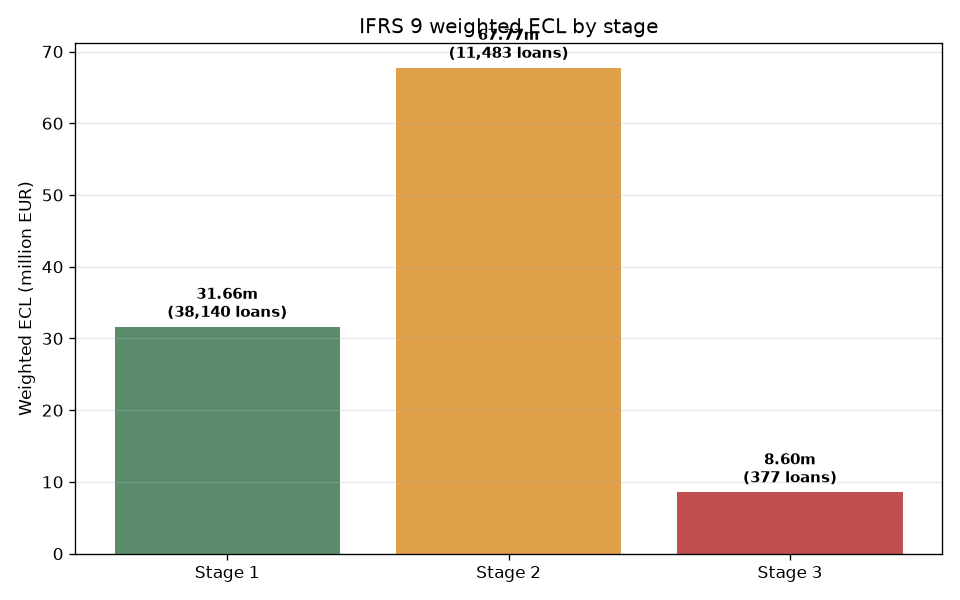
\includegraphics[width=0.85\textwidth]{02_ecl_by_stage.png}
\caption{Weighted ECL by IFRS 9 stage. The middle stage carries the
largest absolute provision, which is the standard shape for IFRS 9
retail books because the lifetime multiplier on non-defaulted-but-
deteriorated exposures compounds a lot of provisioning weight.}
\end{figure}

\begin{figure}[H]
\centering
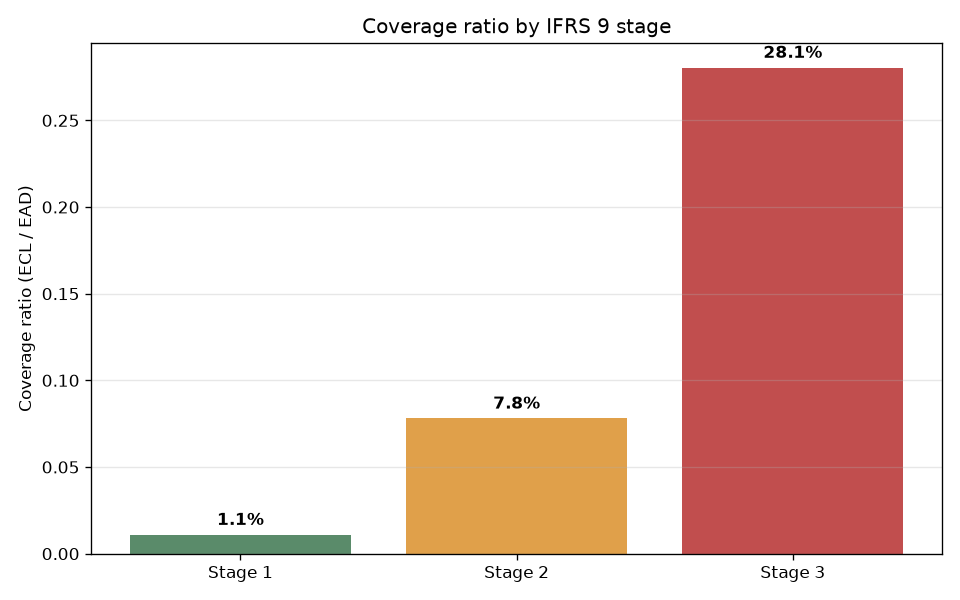
\includegraphics[width=0.85\textwidth]{03_coverage_by_stage.png}
\caption{Coverage ratio (weighted ECL / EAD) by stage. The
approximately 8x step from stage 1 to stage 2, and the further 3.6x
step to stage 3, quantifies the "cliff effect" that IFRS 9 policy
teams monitor closely.}
\end{figure}

\subsection{ECL by product}

\begin{table}[H]
\centering
\begin{tabular}{l r r r r}
\toprule
\textbf{Product} & \textbf{Total EAD (m)} & \textbf{Weighted ECL (m)} & \textbf{Coverage} & \textbf{PD $\times$ LGD baseline} \\
\midrule
Mortgage       & 3\,399.5 & 66.2 & 1.95\%  & 0.57\% \\
Auto           & 167.7   & 10.2 & 6.08\%  & 2.12\% \\
Personal loan  & 112.1   & 16.4 & 14.65\% & 5.82\% \\
Credit card    & 71.6    & 10.1 & 14.10\% & 6.82\% \\
Overdraft      & 29.7    & 5.1  & 17.25\% & 8.73\% \\
\bottomrule
\end{tabular}
\caption{ECL by product. Mortgages carry the largest absolute ECL
due to volume; overdrafts carry the highest coverage ratio due to
combined high PD and high LGD.}
\end{table}

\begin{figure}[H]
\centering
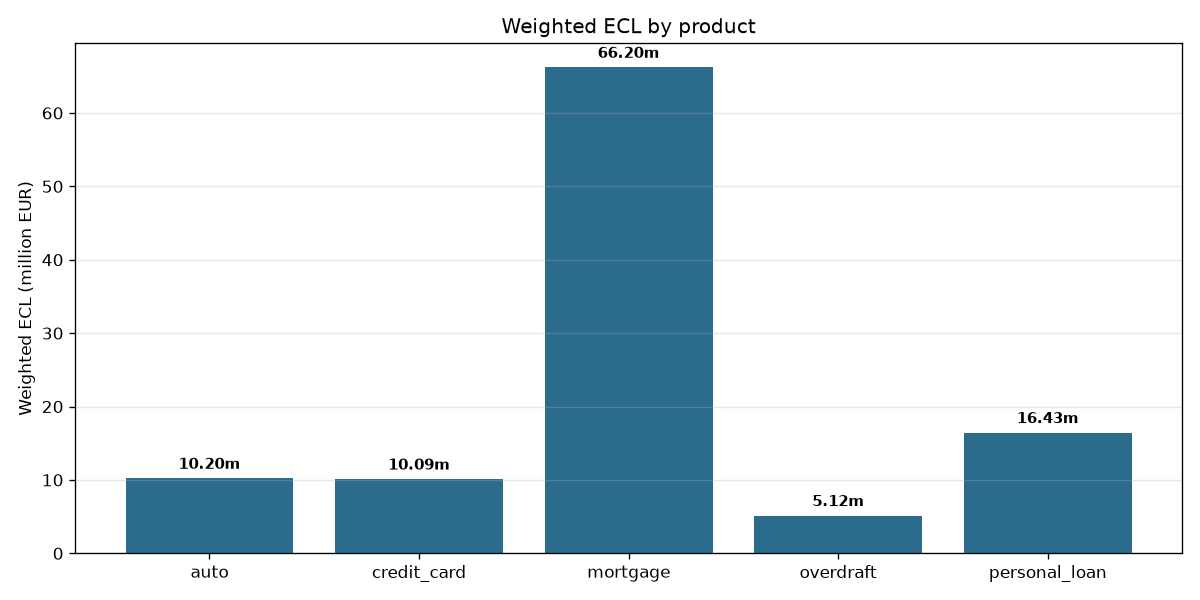
\includegraphics[width=0.9\textwidth]{04_ecl_by_product.png}
\caption{Weighted ECL by product. Mortgage dominates absolute
provisioning; unsecured revolving products dominate coverage
percentages.}
\end{figure}

\subsection{Scenario sensitivity}

\begin{figure}[H]
\centering
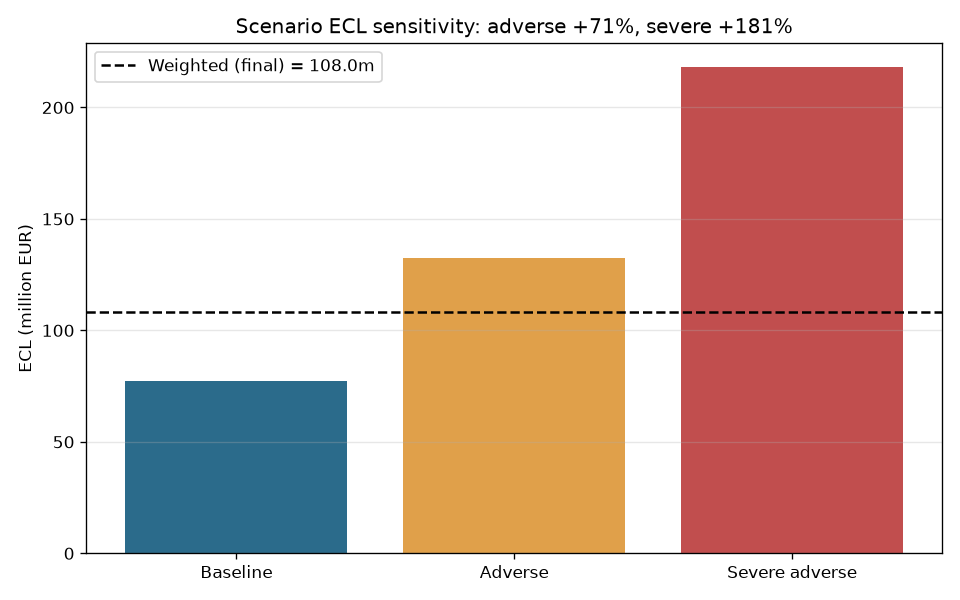
\includegraphics[width=0.85\textwidth]{05_scenario_sensitivity.png}
\caption{Portfolio ECL across the three macro paths with the
weighted line overlaid. The adverse scenario roughly doubles the
baseline provision; severe adverse triples it. The weighted line
sits closer to the baseline because the 60\%-weight baseline
dominates the linear combination.}
\end{figure}

\subsection{Stage-migration cliff}

A recurring question in IFRS 9 is: how much would provisions
jump if a stage-1 loan migrated to stage 2? For every performing
stage-1 loan we compute its hypothetical stage-2 ECL (lifetime PD
$\times$ LGD $\times$ EAD, lifetime-discounted) and compare against
its stage-1 ECL (12-month).

\begin{figure}[H]
\centering
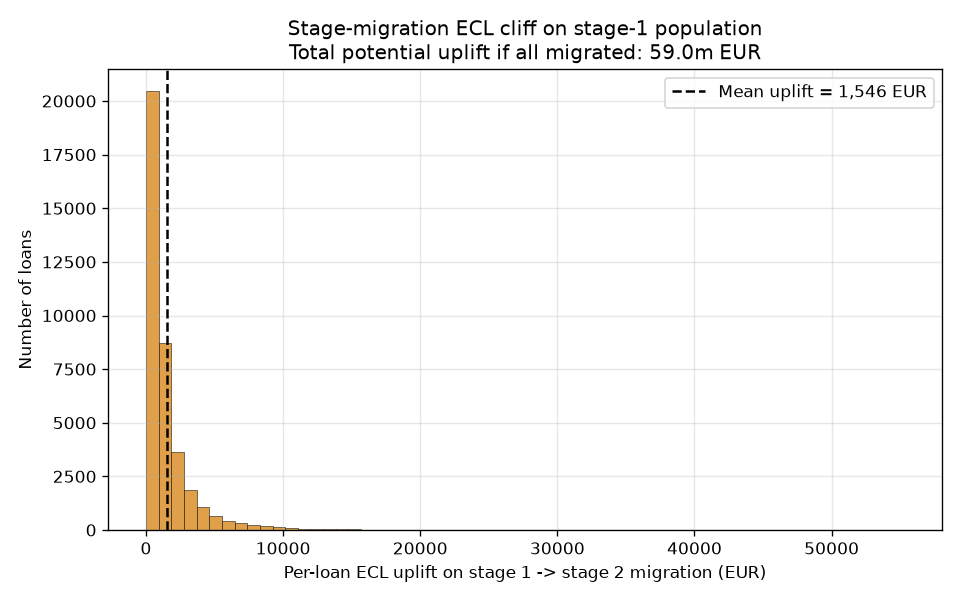
\includegraphics[width=0.85\textwidth]{06_migration_cliff.png}
\caption{Distribution of per-loan ECL uplift if a stage-1 loan
migrates to stage 2. Mean uplift is 1{,}546 EUR per loan. If all
stage-1 loans migrated, total provisions would rise by 59m EUR
(+55\% over the current weighted total). This distribution is what
sensitivity dashboards report to the CFO under IFRS 9 governance.}
\end{figure}

\section{IFRS 9 fit}

\begin{itemize}
  \item \textbf{Point-in-Time (PIT) PD:} The macro-conditional PD
        multipliers deliver a PIT PD by scenario, which is the IFRS 9
        prescription (as opposed to Through-The-Cycle PD used for
        Basel IRB capital).
  \item \textbf{Forward-looking macro:} Three scenarios with fixed
        weights and stress multipliers produce the probability-weighted
        provision required by IFRS 9.5.5.17.
  \item \textbf{Stage 1 (12m) vs Stage 2/3 (lifetime):} Correctly
        distinguished, with stage 3 assigned $\mathrm{PD} = 1$.
  \item \textbf{Discounting to reporting date:} Applied at 3\%
        effective rate.
  \item \textbf{Not fully compliant on:} the macro scenarios are
        deterministic multipliers; a production framework would use
        stochastic simulation of macro paths and rebuild the
        term-structure of PD conditional on each simulated path.
        Discount rate should be the effective interest rate at
        origination, not a portfolio average.
\end{itemize}

\section{Limitations}

\begin{itemize}
  \item PD, LGD, and EAD are treated as independent per-loan draws.
        In reality all three are correlated with the same macro
        state, which produces higher tail ECL than the multiplicative
        stress applied here.
  \item Lifetime PD uses a constant-hazard approximation across
        remaining maturity. A production term-structure model would
        estimate age-dependent hazards.
  \item Behavioural revolving-limit dynamics (limit changes over
        time, borrower requesting increases) are not modelled.
  \item No collateral value re-appraisal over the lifetime horizon.
  \item Stage classification is snapshot-based; a lifetime measurement
        requires modelling stage-migration probabilities.
\end{itemize}

\section{Files}

\begin{itemize}
  \item \texttt{generate\_portfolio.py} --- synthetic performing
        portfolio + macro scenarios
  \item \texttt{compute\_ecl.py} --- end-to-end ECL pipeline with
        staging, lifetime PD, discounting, three scenarios, weighting
  \item \texttt{outputs/} --- loan-level ECL, portfolio-level
        aggregates by stage and product
  \item \texttt{figures/} --- six diagnostic plots
\end{itemize}

\end{document}
